%%%%%%%%%%%%%%%%%%%%%%%%%%%%%%%%%%%%%%%%%%%%%%%%%%%%%%%%%%%%%%%%%%%%%%%%%%%%%%%
\chapter{Performance directed scheduling on asymmetric multi-processors}~\label{chap:pds}
%%%%%%%%%%%%%%%%%%%%%%%%%%%%%%%%%%%%%%%%%%%%%%%%%%%%%%%%%%%%%%%%%%%%%%%%%%%%%%%

Current implementations of schedulers in modern operating systems recognize the environment
as homogeneous in nature while technologies such as DVFS (Dynamic Voltage and Frequency Scaling) introduce an
inherent asymmetry in a multiprocessor system. 
Considerable direction in terms of asymmetric scheduling support has been addressed in \cite{AsymmetricScheduling}
and \cite{Multitasking} but on the downside, the work does not consider the requirements of tasks in terms of capability
and speed of the processing element which brings little advantage to the existing system.

In a multi-core environment, there are many facets for performance loss with the most 
common reasons being high IO and memory latencies which is further aggravated by cache sharing.
A novel statistical learning method to predict voltage and frequency requirements by tasks 
was proposed in \cite{AnIntraTask}, but the method required rigorous statistical learning making it 
time consuming and impossible to implement at the context of a scheduler. A
simpler method was proposed in \cite{LiveRuntime} and \cite{Phaseaware}, but comes at the cost
of possible rapid voltage and frequency transitions which may lead to instabilities in emergencies
(Even with a quad core system and a scheduling frequency of 1000Hz, there is a possibility
of $1000 \times 4 = 4000$ performance state transitions every second) as shown in \cite{ImpactDVFS}. 

%%%%%%%%%%%%%%%%%%%%%%%%%%%%%%%%%%%%%%%%%%%%%%%%%%%%%%%%%%%%%%%%%%%%%%%%%%%%%%%
\section{Performance behavior of SPEC workloads}~\label{sec:perf_behav}
%%%%%%%%%%%%%%%%%%%%%%%%%%%%%%%%%%%%%%%%%%%%%%%%%%%%%%%%%%%%%%%%%%%%%%%%%%%%%%%

In order to study the behavior of real applications on different voltage and frequency settings,
fourteen of the SPEC2006 \cite{spec:2006} benchmark suite were run with varied clock speed 
from 1100 MHz to 2200 MHz on an AMD Opteron Quad core processor and were plotted showing the 
percentage duration spent at an IPC (Instruction per Clock) higher than 1.0 and the 
speed-up in terms of execution time achieved from that when run with the lowest clock speed (1100 MHz). 
This is shown in Figure~\ref{fig:spec_classify}.
The X-axis of this graph is the percentage of time the benchmark spent running at an IPC level greater
than 1.0, the Y-axis is the clock speed at which the benchmark was run at, and finally the Z-axis 
is the Speed-up achieved. It can be observed that the return on investment (Higher clock speed)
is low for tasks with a low percentage of runtime at an IPC greater than 1.0. Artificial workloads
comprising of 4 benchmarks each were created (shown in Table~\ref{tab:spec_groups}) based on their IPC classification
and real-world usage on throughput based systems. Figure~\ref{fig:group_speedup} shows that the workload 
\textit{High} category shows the greatest improvement with frequency, achieving a nearly 2x improvement using the highest
frequency for each core in the 4-core system.  Otherwise, the other
categories of workloads appear to benefit from higher frequency, but
are bounded to 1.5x of the baseline execution time.
This motivates the construction of a performance directed scheduler aware of the IPC
level at which tasks are executing and described in further sections. 

\begin{figure}[h!]
  \begin{center}
    %\resizebox{\columnwidth}{!}{
    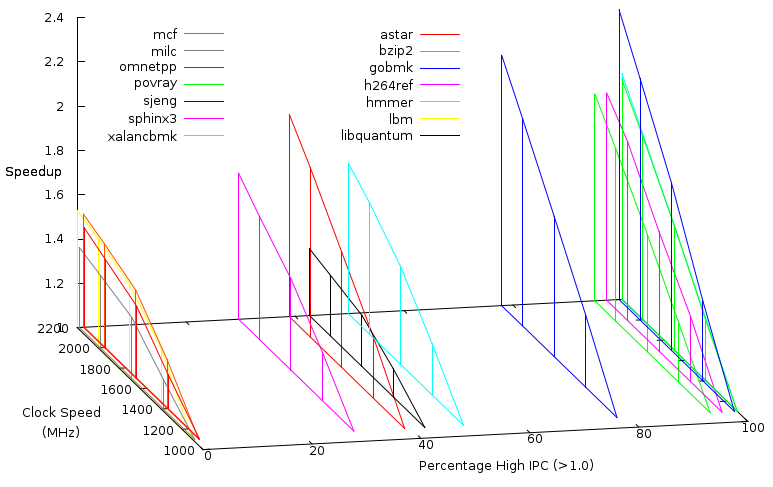
\includegraphics[height=3.5in]{figures/Speedup_Classify.png}%}
    \caption{IPC classification and speedup trends for the SPEC 2006 benchmarks}
    \label{fig:spec_classify}
  \end{center}
\end{figure}

\begin{figure}[h!]
  \begin{center}
    %\resizebox{\columnwidth}{!}{
    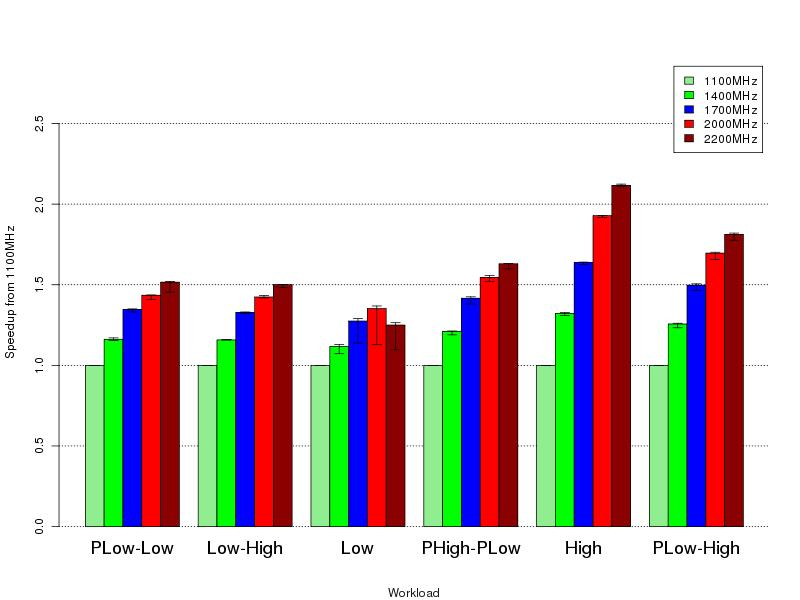
\includegraphics[height=3.5in]{figures/group_speedup.jpg}%}
    \caption{Speedup achieved by characterized workloads}
    \label{fig:group_speedup}
  \end{center}
\end{figure}

%%%%%%%%%%%%%%%%%%%%%%%%%%%%%%%%%%%%%%%%%%%%%%%%%%%%%%%%%%%%%%%%%%%%%%%%%%%%%%%
\section{Quantifying performance}~\label{sec:quant_perf}
%%%%%%%%%%%%%%%%%%%%%%%%%%%%%%%%%%%%%%%%%%%%%%%%%%%%%%%%%%%%%%%%%%%%%%%%%%%%%%%

An adaptive system needs a quantitative measure of performance. Section~\ref{sec:perf_behav} indicated
that IPC can be used as such a measure. In order to study the throughput and energy consumption behavior of
workloads, a hardware monitoring-based framework was constructed to
collect and correlate per-application IPC data. Figure~\ref{fig:ipc_speedup} 
was constructed displaying the speedup which was achieved in terms of throughput when compared to the same 
sample executed at the base clock speed of 1100 MHz. This provides an aid in observing the exact IPC
values at which a higher clock speed is no better in increasing the throughput. Figure~\ref{fig:ipc_speedup}
shows that beyond $IPC = 1.0$, a higher clock speed always provide better throughput to the system. On the
other hand, at $IPC < 0.75$ going from 2000MHz to 2200MHz exhibit absolutely no additional throughput 
and this observation continues as IPC reduces beyond 0.5.

\begin{figure}[h!]
  \begin{center}
    %\resizebox{\columnwidth}{!}{
    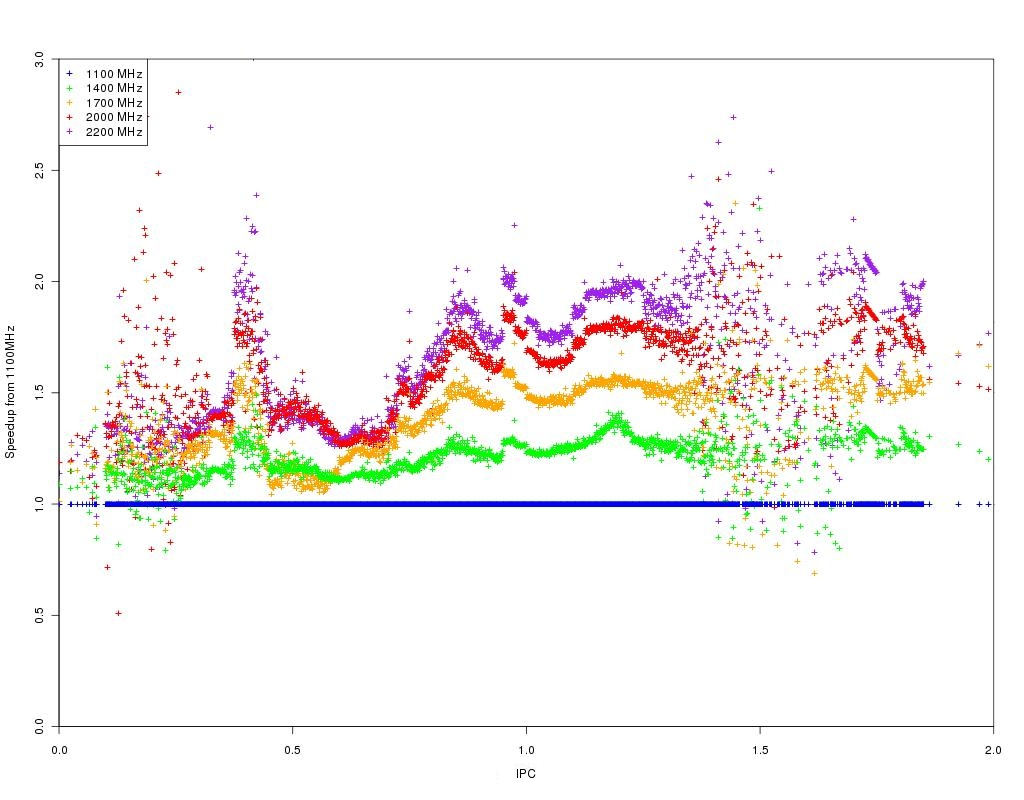
\includegraphics[height=3in]{figures/ipc_speedup.jpg}%}
    \caption{Speedup dependence with IPC}
  \end{center}
  \label{fig:ipc_speedup}
\end{figure}

By reducing clock speed (and hence power consumption), it can be hypothesized that the execution time
increases proportionally and hence maintaining the total energy consumption.
Figure~\ref{fig:ipc_epi} validates this claim that 
the energy consumption per instruction (EPI) is invariant of clock speed, except at lower IPC levels
where lower clock speeds demonstrate better EPI behavior.

\begin{figure}[h!]
  \begin{center}
    %\resizebox{\columnwidth}{!}{
    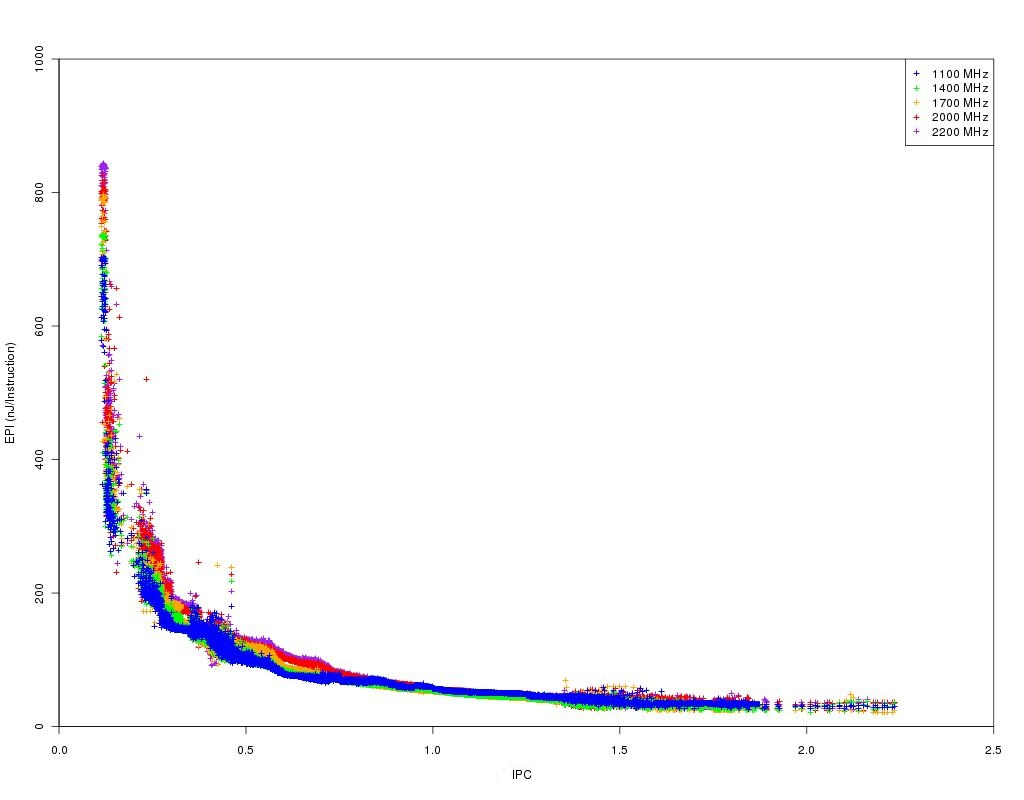
\includegraphics[height=3in]{figures/ipc_epi.jpg}%}
    \caption{Energy consumption per instruction variance with IPC}
    \label{fig:ipc_epi}
  \end{center}
\end{figure}

%%%%%%%%%%%%%%%%%%%%%%%%%%%%%%%%%%%%%%%%%%%%%%%%%%%%%%%%%%%%%%%%%%%%%%%%%%%%%%%
\section{Hierarchical processor organization}~\label{sec:proc_org}
%%%%%%%%%%%%%%%%%%%%%%%%%%%%%%%%%%%%%%%%%%%%%%%%%%%%%%%%%%%%%%%%%%%%%%%%%%%%%%%

Sections \ref{sec:perf_behav} and \ref{sec:quant_perf}  provide a strong motivation to
scale voltage and frequency of processors based on the performance of the workload.
While most of the research pertaining to workload based DVFS direct their attention of changing the voltage and frequency levels
based on the task's demand, none consider the possibility that such a performance state might
already be available on another core which can be remedied by a simple migration without the 
causality of rapid performance state transitions. The motivation to substitute migration to
a frequency transition is further enhanced with the current multi-core race where the probability
of such a situation improves proportionally.  

In order to enable scheduling on asymmetric multiprocessors, the first implementation
step was to organize the processor set as groups with equal performance states. 
The term performance state or P-State will be used to differentiate varied voltage and
frequency configurations which a processor is allowed to have, and is indicated by
$P_{0}$ through $P_{M-1}$ where, $P_0$ is the configuration with the lowest clock speed
and voltage (In effect a lower power consumption). Each set maintains the usage in terms
of actively running tasks in the particular group to enable load balancing between 
groups of varied performance states. This view of the processor set is shown in
Figure~\ref{fig:processor_groups} and mathematically viewed as a vector of sets shown in Figure~\ref{fig:layout_scheduler}.
Here, $C_{P_{i}}$ is the set of processors which are at 
a performance state of $P_{i}$. Individual processor cores are represented as $C_{i}$.


\begin{figure}[h!]
  \begin{center}
%    \resizebox{\columnwidth}{!}{
    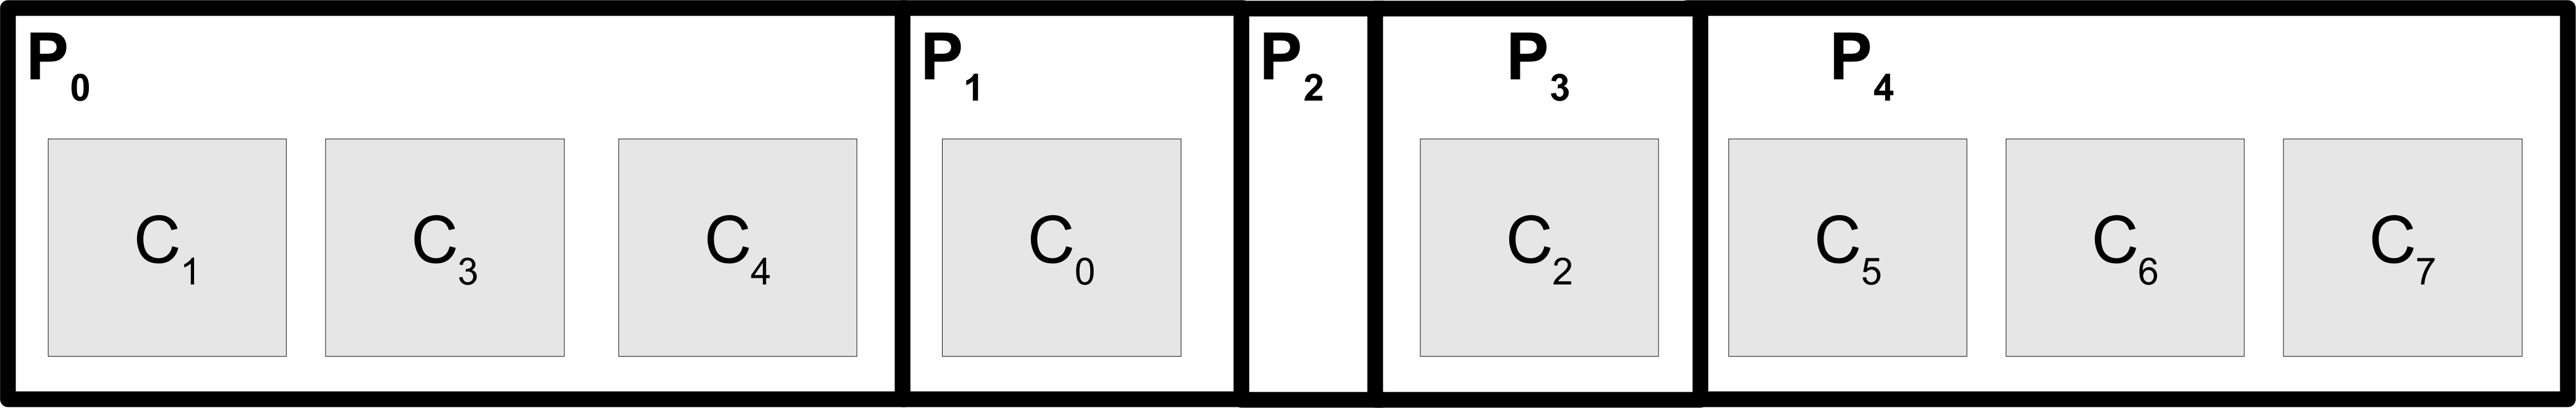
\includegraphics[height=1in]{figures/Processor_Organization.jpg}%}
    \caption{Multi-processor organization}
    \label{fig:processor_groups}
  \end{center}
\end{figure}

\begin{figure}[h!]
\centering
\begin{equation*}
   L^{s} = \left[
     \begin{array}{lccr}
       C_{P_{0}} & C_{P_{1}} & ... & C_{P_{M-1}}
     \end{array} \right]
\end{equation*}
\caption{Definition of the processor layout with M performance states}
\label{fig:layout_scheduler}
\end{figure}


%%%%%%%%%%%%%%%%%%%%%%%%%%%%%%%%%%%%%%%%%%%%%%%%%%%%%%%%%%%%%%%%%%%%%%%%%%%%%%%
\section{Hardware performance counters}~\label{sec:perf_counters}
%%%%%%%%%%%%%%%%%%%%%%%%%%%%%%%%%%%%%%%%%%%%%%%%%%%%%%%%%%%%%%%%%%%%%%%%%%%%%%%

In order to quantitatively measure the performance of each task, 
a driver was developed to read and configure the hardware performance counters
present in the AMD and Intel Architectures. Two counters one to count retired instructions
while another to count real clock cycles were configured to measure the sample IPC 
of an executing workload as shown in Figure~\ref{fig:hw_counters}. Every
request for IPC made to the performance monitoring subsystem, the current value of 
both counters are read, and based on which the IPC is computed and returned to the consumer
as a fixed point value with the lower three bits containing the fraction (a precision 
of 0.125). After every successful transaction, the counters are cleared and continue incrementing with each event.
The performance monitoring subsystem is unaware of the current executing task and it is the scheduler's
responsibility to read the IPC level before switching out tasks form the running state. 

\begin{figure}[h!]
  \begin{center}
    %\resizebox{\columnwidth}{!}{
    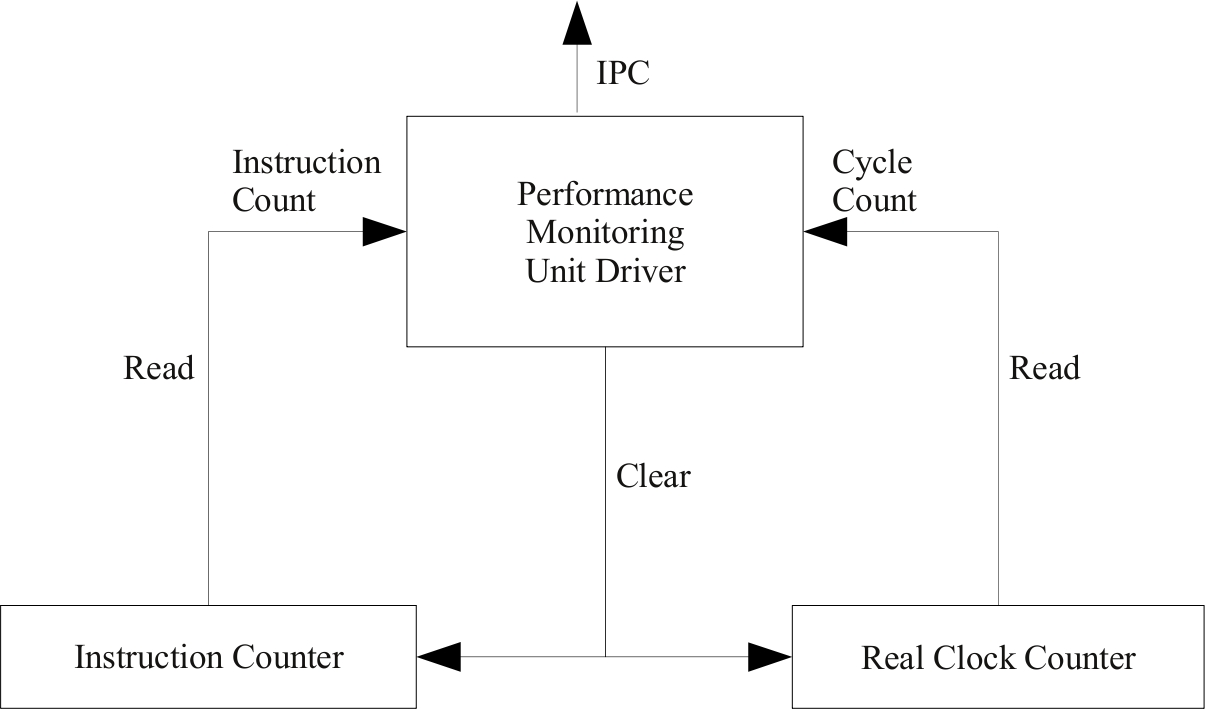
\includegraphics[height=2in]{figures/HW_Counter.jpg}%}
    \caption{Hardware performance monitoring counters}
    \label{fig:hw_counters}
  \end{center}
\end{figure}

%%%%%%%%%%%%%%%%%%%%%%%%%%%%%%%%%%%%%%%%%%%%%%%%%%%%%%%%%%%%%%%%%%%%%%%%%%%%%%%
\section{Scheduling methodology}~\label{sec:pds}
%%%%%%%%%%%%%%%%%%%%%%%%%%%%%%%%%%%%%%%%%%%%%%%ttf-opensymbol%%%%%%%%%%%%%%%%%%%%%%%%%%%%%%%%

It is common for the number of tasks in the ready state to be greater than the total number
of processors. Most time sharing scheduling systems regularly switch out a running task
to another in order to provide fair equal execution times for all tasks. This execution slice is commonly 
referred to as the scheduling quanta. The Linux Scheduling system, in order to support symmetric 
multi-processor environments, maintains separate run-queues
for each processing element. As a direct consequence, the scheduling state diagram is replicated for each processor. 
Migration, a procedure of moving a runnable task from one processor to another is reduced to migrating the task from
one run-queue to another. 

Figure~\ref{fig:pds_method} shows the state diagram of the performance directed scheduler which is a modification of
the default Linux scheduler with an additional pseudo state (Performance directed Migration) introduced at the transition 
away from the running state (This is termed as a pseudo state as it is just a place holder to describe the arcs at 
which performance directed decisions are made). At this state as shown in Figure~\ref{fig:pds_migration}, the hardware 
performance counters are queried for the value of the current IPC (Instructions per clock). 
Based on this quantitative measure of the task's performance,
a mapping from IPC to a required performance state ($P'$) is made. This mapping can potentially be done is a number of ways 
of which two were implemented and evaluated and described in the following two subsections. Once $P'$ is estimated, 
the layout $L^s$ is is queried for the total number of processors in the set $C_{P'}$ and the total number of tasks in the 
ready or running state for processors in $C_{P'}$. If the set $C_{P'}$ is populated or the total number of tasks executing 
on the processors in set $C_{P'}$ is lesser than or equal
to the number of processors in $C_{P'}$, then $P'' = P'$. But if such is not the case, then the layout $L^s$ is searched
for a set $C_{P''}$ such that $P''$ is closest to $P'$, and $C_{P''}$ is populated and the total number of tasks 
executing in the set $C_{P''}$ is lesser than the number of processors in $C_{P''}$. If all fails, then the layout
is searched for a state $P''$ such that $C_{P''}$ is populated and the load (Computed as the total number of tasks 
divided by the number of processors) is minimum. Decisions on the exact processor a task has to execute on is made by the 
underlying native scheduler of the operating system and the PDS is completely oblivious to any further details.
As an interface to the mutator which will be explained in Chapter~\ref{chap:delta}, PDS
increments the cell corresponding to $P'$ in the demand vector \textbf{D} ($D_{P'} = D_{P'} + 1$).

\begin{figure}[h!]
  \begin{center}
%    \resizebox{\columnwidth}{!}{
    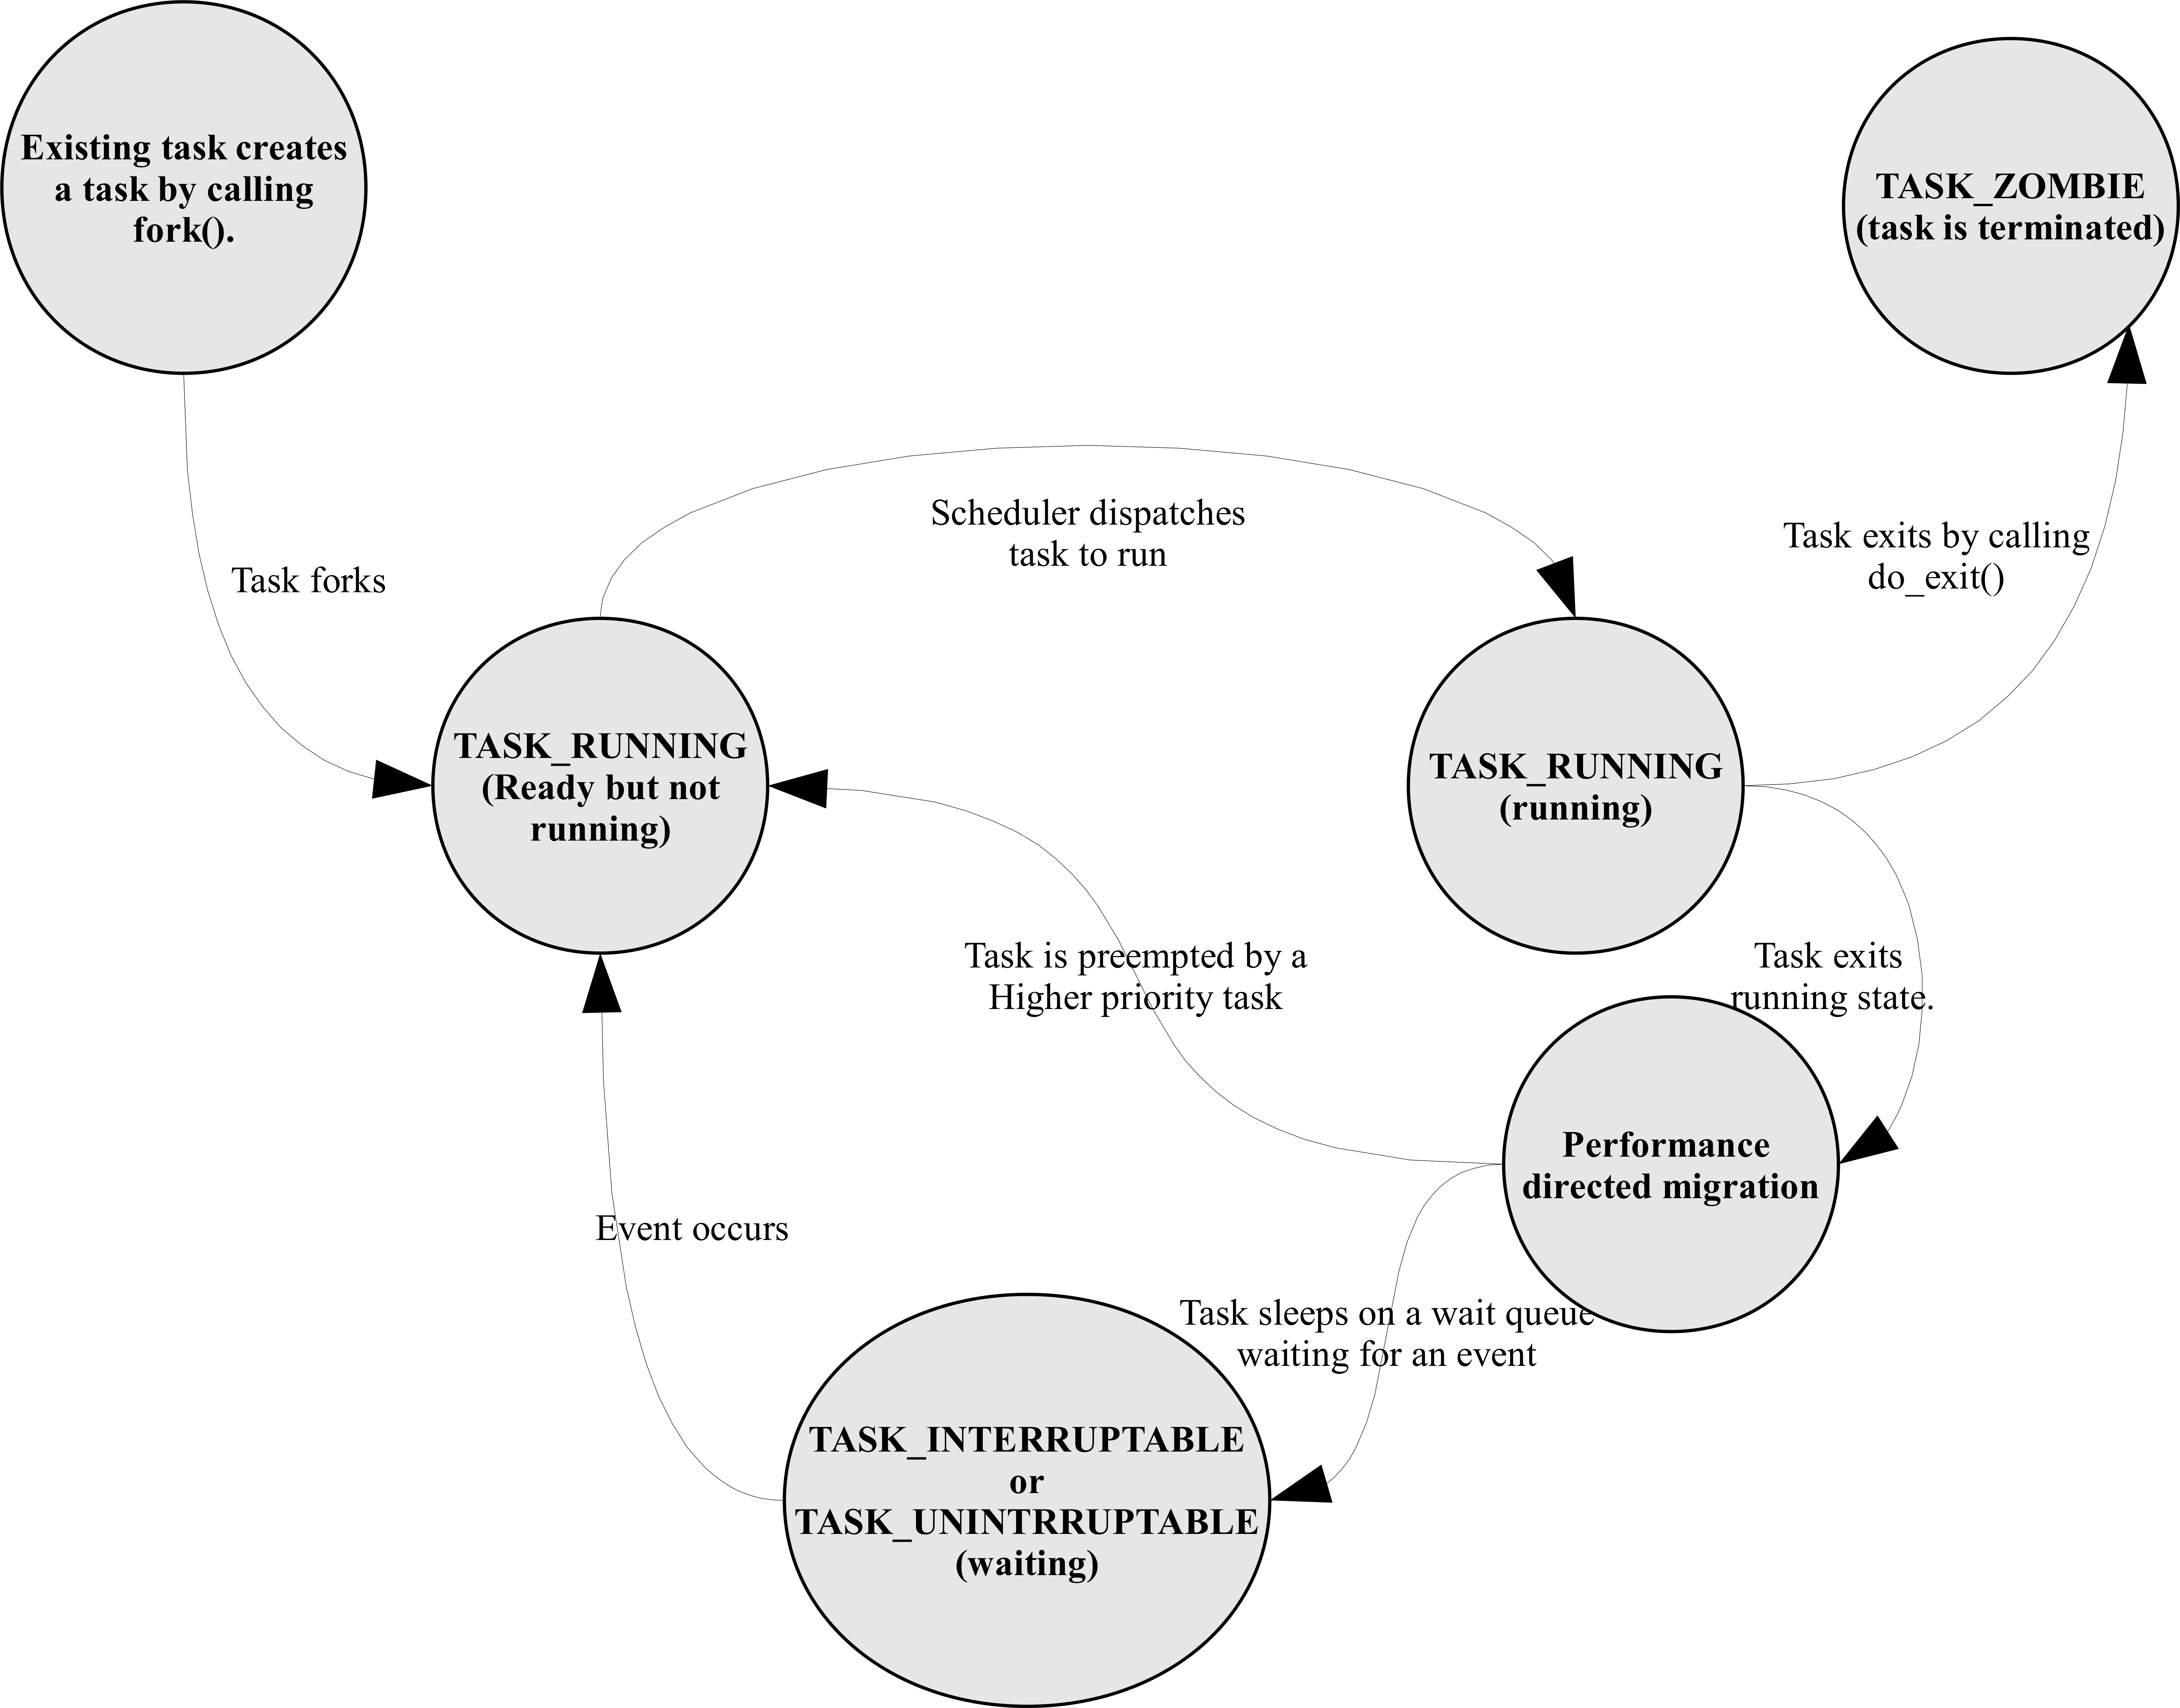
\includegraphics[height=3in]{figures/Mod_Linux_Sched.jpg}%}
    \caption{Scheduling state diagram}
    \label{fig:pds_method}
  \end{center}
\end{figure}

\begin{figure}[h!]
  \begin{center}
    \resizebox{\columnwidth}{!}{
    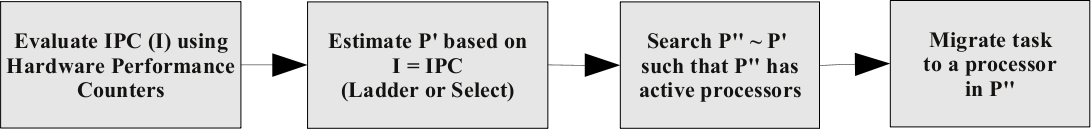
\includegraphics{figures/Migration.jpg}}
    \caption{Performance directed migration}
    \label{fig:pds_migration}
  \end{center}
\end{figure}


%%%%%%%%%%%%%%%%%%%%%%%%%%%%%%%%%%%%%%%%%%%%%%%%%%%%%%%%%%%%%%%%%%%%%%%%%%%%%%%
\subsection{Ladder performance state estimation}~\label{sec:ladder}
%%%%%%%%%%%%%%%%%%%%%%%%%%%%%%%%%%%%%%%%%%%%%%%%%%%%%%%%%%%%%%%%%%%%%%%%%%%%%%%

The ladder performance state estimation sports a simple decision procedure. If $IPC > H$ 
where \textbf{H} is set to 0.875, then $P'$ is chosen such that is is higher than the state
at which the task is currently executing with ($P' = P + 1$). If $IPC < L$ ($L = 0.5$), then 
$P'$ is chosen to be one less than the state at which the task is executing with ($P' = P - 1$). 
Otherwise the $P'$ is chosen to be equal to $P$. The advantage of the procedure is the lower
choice (two: H and L) available to the system administrator. It is clear that the wrong choice of these
thresholds can cause undesirable power and performance behavior of the system. These thresholds are
selected based on the graph shown in Figure~\ref{fig:ipc_speedup}. 

\begin{figure}[h!]
  \begin{center}
%    \resizebox{\columnwidth}{!}{
    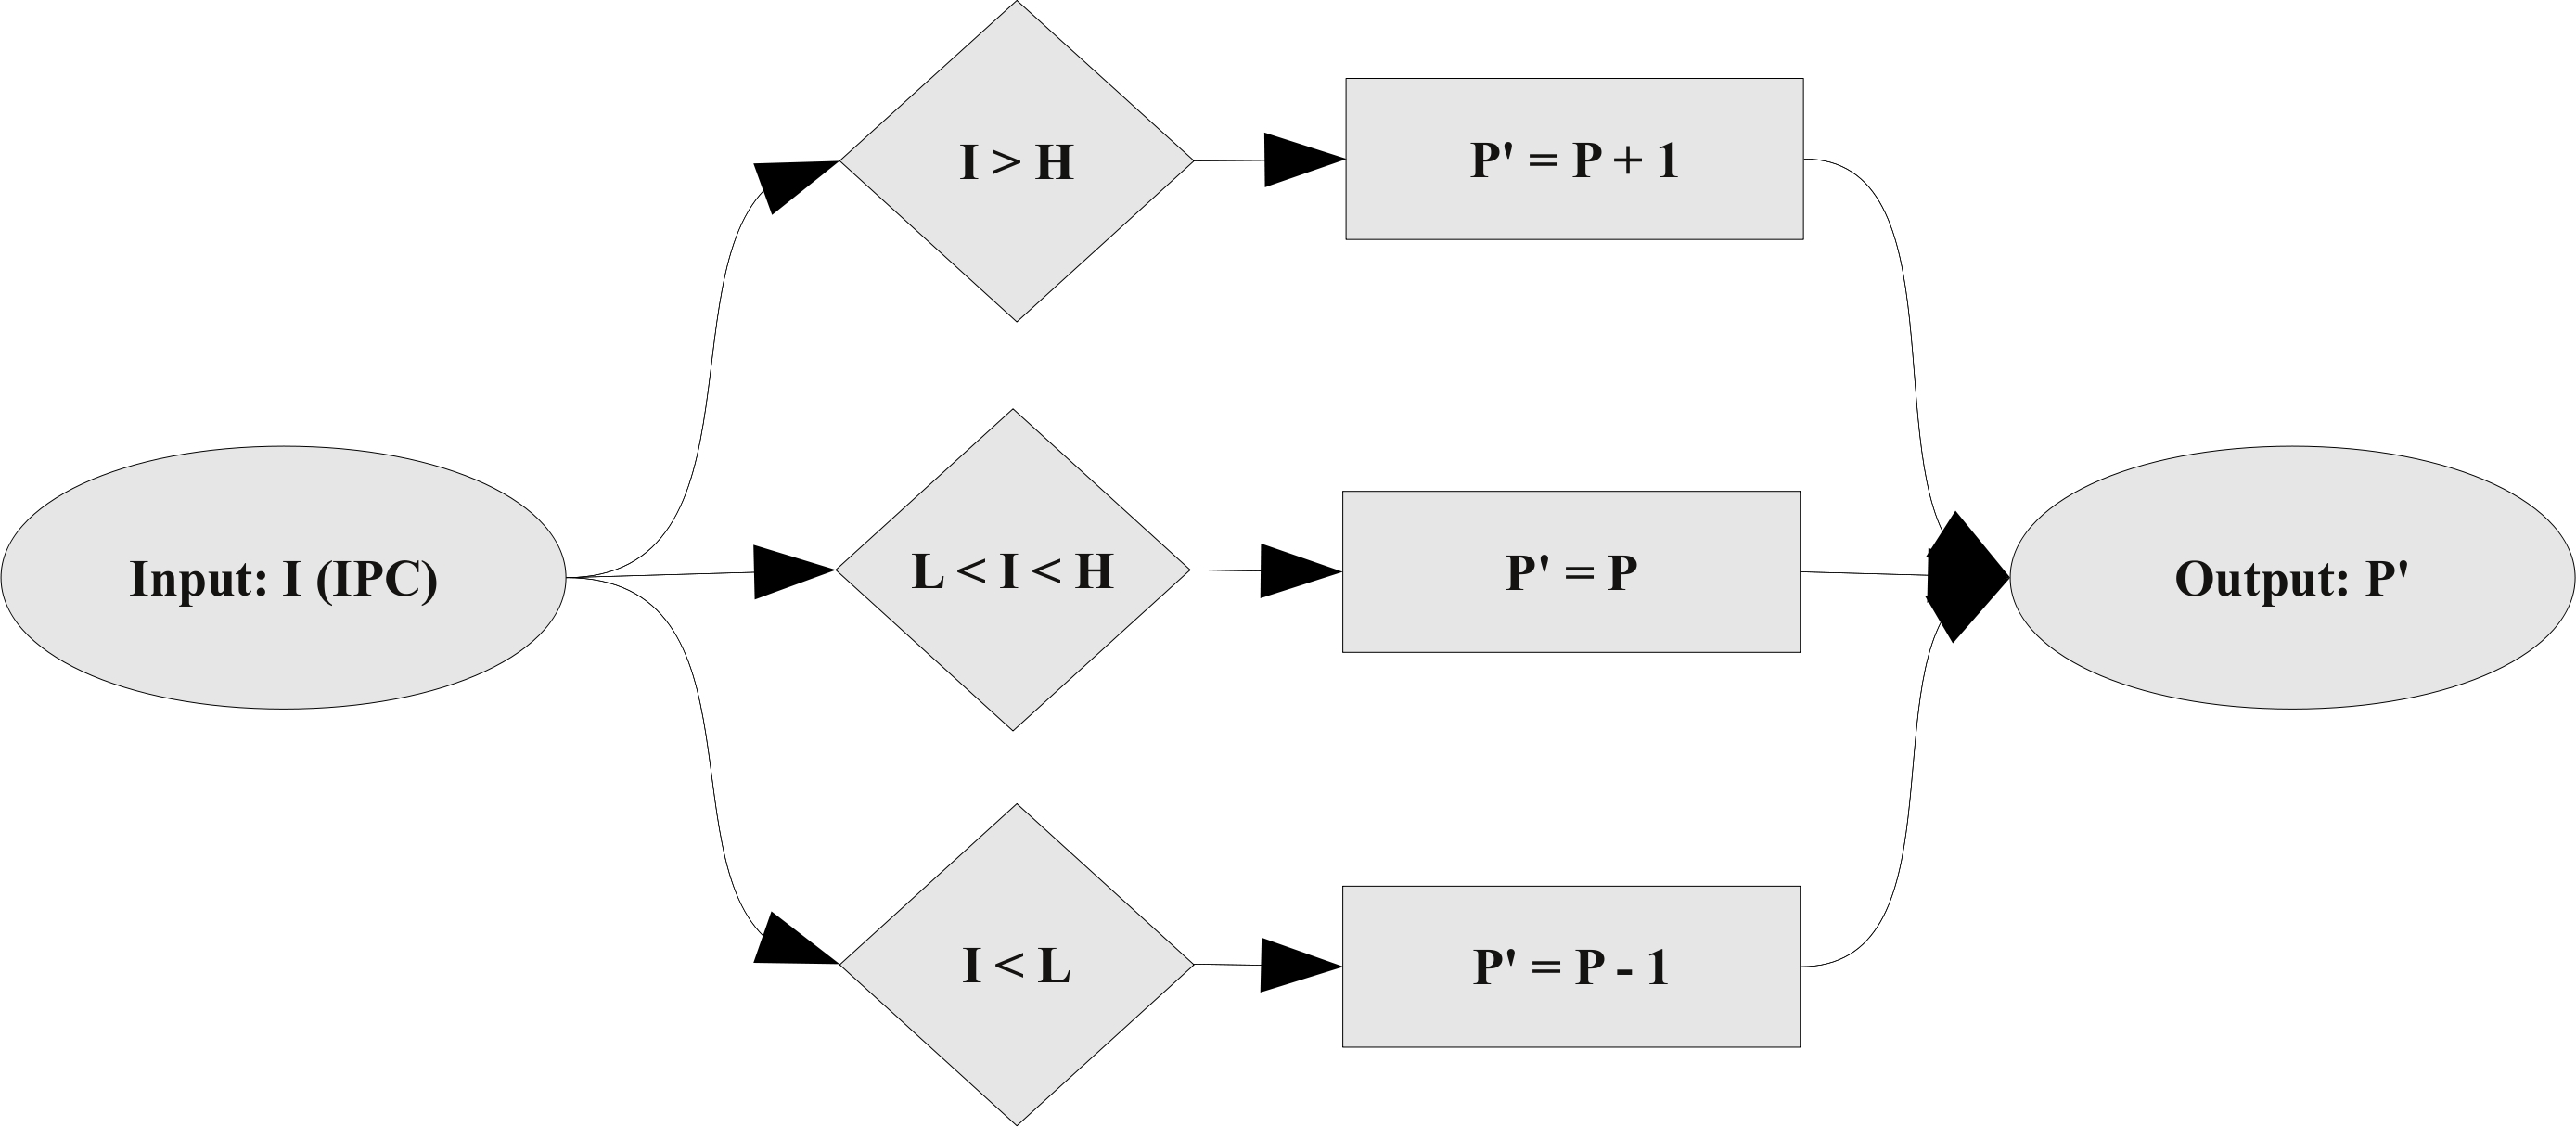
\includegraphics[height=2in]{figures/Ladder_Evaluation.jpg}%}
    \caption{Ladder performance state estimation algorithm}
    \label{fig:ladder_method}
  \end{center}
\end{figure}

%%%%%%%%%%%%%%%%%%%%%%%%%%%%%%%%%%%%%%%%%%%%%%%%%%%%%%%%%%%%%%%%%%%%%%%%%%%%%%%
\subsection{Select performance state estimation}~\label{sec:select}
%%%%%%%%%%%%%%%%%%%%%%%%%%%%%%%%%%%%%%%%%%%%%%%%%%%%%%%%%%%%%%%%%%%%%%%%%%%%%%%

A logical extension of the ladder estimation, is the select estimation shown in Figure~\ref{fig:select_method}.
This is when, a performance state is fixed for each range of IPC. Such a system was implemented with 
threshold values shown in Table~\ref{tab:sel_threshold}. This system was evaluated along with
the ladder evaluation with the delta based mutation described in Chapter~\ref{chap:delta}.

\begin{figure}[h!]
  \begin{center}
%    \resizebox{\columnwidth}{!}{
    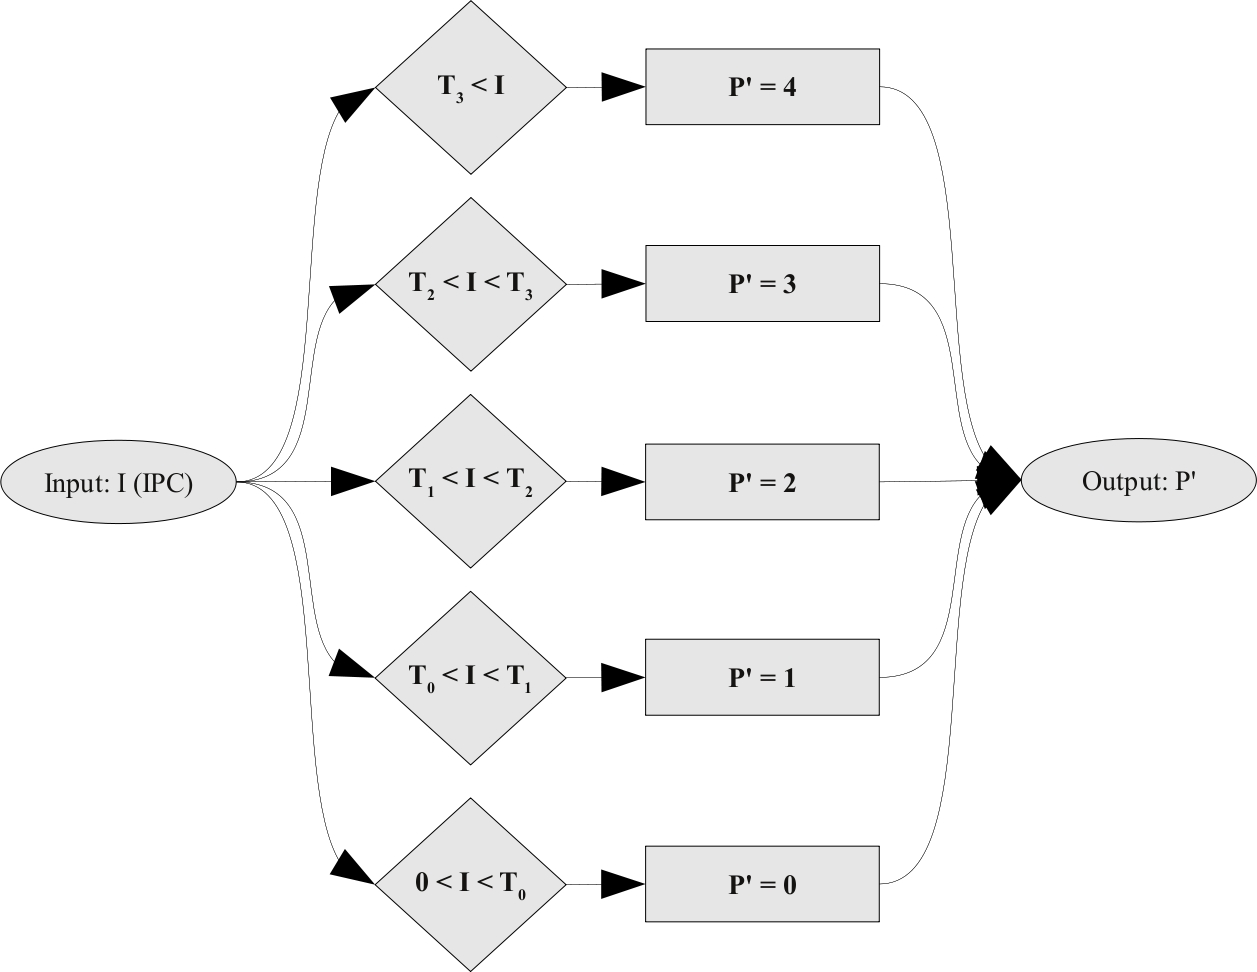
\includegraphics[height=3in]{figures/Select_Evaluation.jpg}%}
    \caption{Select performance state estimation algorithm}
    \label{fig:select_method}
  \end{center}
\end{figure}

\begin{table}[h!]
 \begin{center}
\begin{tabular}{| l | l | }
\hline	
Threshold & Value \\
\hline
$T_0$ & 0.25  \\
$T_1$ & 0.50  \\
$T_2$ & 0.75  \\
$T_3$ & 1.25  \\
\hline  
\end{tabular}
 \end{center}
\caption{Threshold values for the select evaluation}
\label{tab:sel_threshold}
\end{table}


%%%%%%%%%%%%%%%%%%%%%%%%%%%%%%%%%%%%%%%%%%%%%%%%%%%%%%%%%%%%%%%%%%%%%%%%%%%%%%%
\section{Experimental setup}~\label{sec:pds_exp}
%%%%%%%%%%%%%%%%%%%%%%%%%%%%%%%%%%%%%%%%%%%%%%%%%%%%%%%%%%%%%%%%%%%%%%%%%%%%%%%

The experiments were conducted on a AMD quad-core Barcelona which allows individual
processor cores to be set to different clock speeds. Different synthetic workloads
based on real world usages were set up using the SPEC2006 benchmarks and classified based on their IPC. The 
individual members of each group are provided in Appendix~\ref{app:benchmark}. The workload was started
on the layouts provided in Table~\ref{tab:proc_layouts}, and the execution time of each
member benchmark was measured and summed to arrive at a single execution time per 
workload. The experiment was repeated multiple times and the mean of the execution times were 
compared with that of the $[4,4,4,4]$ layout to get the percentage slow down. 
The results are shown in Figure~\ref{fig:fixed_res}.  

\begin{table}[h!]
 \begin{center}
\begin{tabular}{| l | l | l | l | l | }
\hline	
Layout Name & $P_{C_{0}}$ & $P_{C_{1}}$ & $P_{C_{2}}$ & $P_{C_{3}}$ \\
\hline
a & 0 & 0 & 0 & 0 \\
b & 0 & 0 & 1 & 1 \\
c & 0 & 0 & 2 & 2 \\
d & 0 & 0 & 0 & 4 \\
e & 1 & 1 & 2 & 2 \\
f & 0 & 0 & 3 & 3 \\
g & 0 & 0 & 4 & 4 \\
h & 1 & 1 & 3 & 3 \\
i & 1 & 1 & 4 & 4 \\
j & 2 & 2 & 3 & 3 \\ 
k & 2 & 2 & 4 & 4 \\ 
l & 0 & 4 & 4 & 4 \\
m & 3 & 3 & 4 & 4 \\
n & 4 & 4 & 4 & 4 \\
\hline  
\end{tabular}
 \end{center}
\caption{Experimental layouts}
\label{tab:proc_layouts}
\end{table}

\begin{figure}[h!]
  \begin{center}
    %\resizebox{\columnwidth}{!}{
    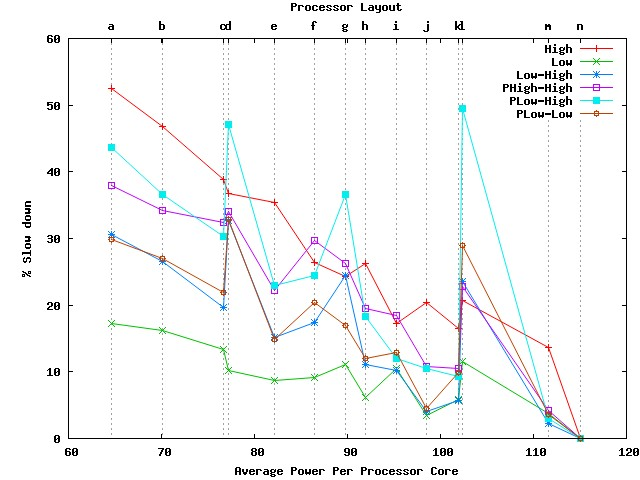
\includegraphics[height=4in]{figures/fixed_results.jpg}%}
    \caption{Slowdown vs power consumption for fixed layouts}
    \label{fig:fixed_res}
  \end{center}
\end{figure}

One obvious trend is decrease in the percentage slowdown with the increase of power provided per 
core (Higher performance states available)
increases. The problem with fixed static layouts are obvious from the peaks observed
whenever there is an asymmetry in the layout for example $[0,0,0,4]$ where processor
$C_3$ is in state $P_4$ while the remaining processors $C_0$,$C_1$ and $C_2$ are in
$P_0$. A particular time line for such a configuration is shown in Figure~\ref{fig:fight_to_death}.
The reason for the spikes become fairly obvious from the rapid migrations observed for
a fairly stable phased behavior. This is usually common when there are more tasks battling
over a lower number of processors where the time spent in migrations
become noticeable and add to the slow down of the task. 



\begin{figure}[h!]
  \begin{center}
    %\resizebox{\columnwidth}{!}{
    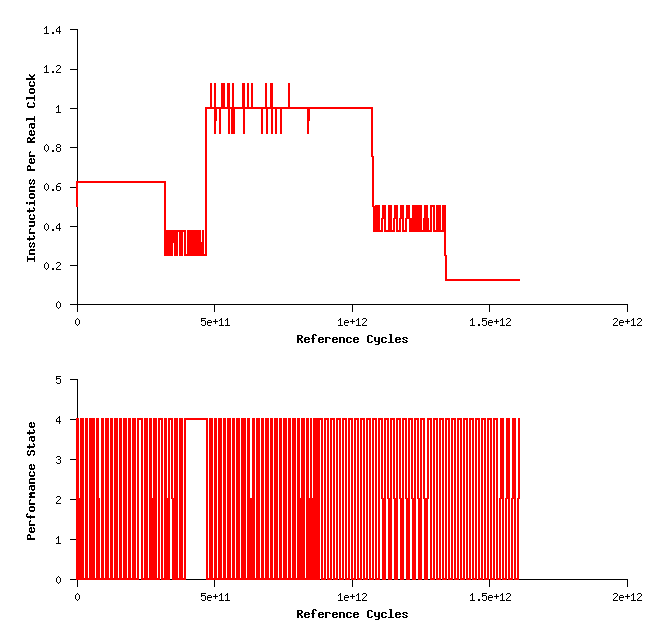
\includegraphics[height=3in]{figures/astar_fight.png}%}
    \caption{Astar running on a $[0,0,0,4]$ layout}
    \label{fig:fight_to_death}
  \end{center}
\end{figure}
